\documentclass[14pt]{beamer}


\usepackage{color}
\usepackage{tikz}


\mode<presentation>
{
\usetheme{AlpesLasers}
\setbeamercovered{transparent}
  %\setbeamertemplate{footline}[frame number] 
  %\setbeamertemplate{navigation symbols}{ 
  %\hskip 0.3cm
  %\insertframenumber / \inserttotalframenumber  % <<< frame #
  %\insertpagenumber / \insertpresentationendpage % <<< page #
%} 
}

% font definitions, try \usepackage{ae} instead of the following
% three lines if you don't like this look
\usepackage{listings}
\lstloadlanguages{python}

\usepackage{mathptmx}
\usepackage[scaled=.90]{helvet}
\usepackage{courier}
\usepackage[T1]{fontenc}
\usepackage[english]{babel}
\usepackage[latin1]{inputenc}
\title{ALDIRAC}
\subtitle{status / future}
\author{St\'ephane Poss}
\date{\today}
% This is only inserted into the PDF information catalog. Can be left
% out.
\subject{PYTHON}

\begin{document}
\begin{frame}[plain]
\titlepage
\end{frame}

\begin{frame}
\tableofcontents
\end{frame}

\section{ALDIRAC}
\begin{frame}
\frametitle{ALDIRAC status}
Uses:
\begin{itemize}
\item DIRAC v6r11p23
\pause
\item VMDIRAC v1r0, patched for AWS
\end{itemize}
~\\
\pause
Adds dedicated system to manage Alpes~Lasers data (SimuDB)
\end{frame}

\begin{frame}
\frametitle{Run framework}
Use AWS:
\begin{itemize}
\item image created once, stored on AWS
\item ALDIRAC update performed at boot time using dedicated tool
\end{itemize}
Software management:
\begin{itemize}
\item AL software only in AL premises
\item rsync'ed with ssh at job start
\item Mostly uses 'pip' package structure $\rightarrow$ easy installation
\end{itemize}
\end{frame}

\section{ALDIRAC system: SimuDB}
\begin{frame}
\frametitle{SimuDB}
\centering
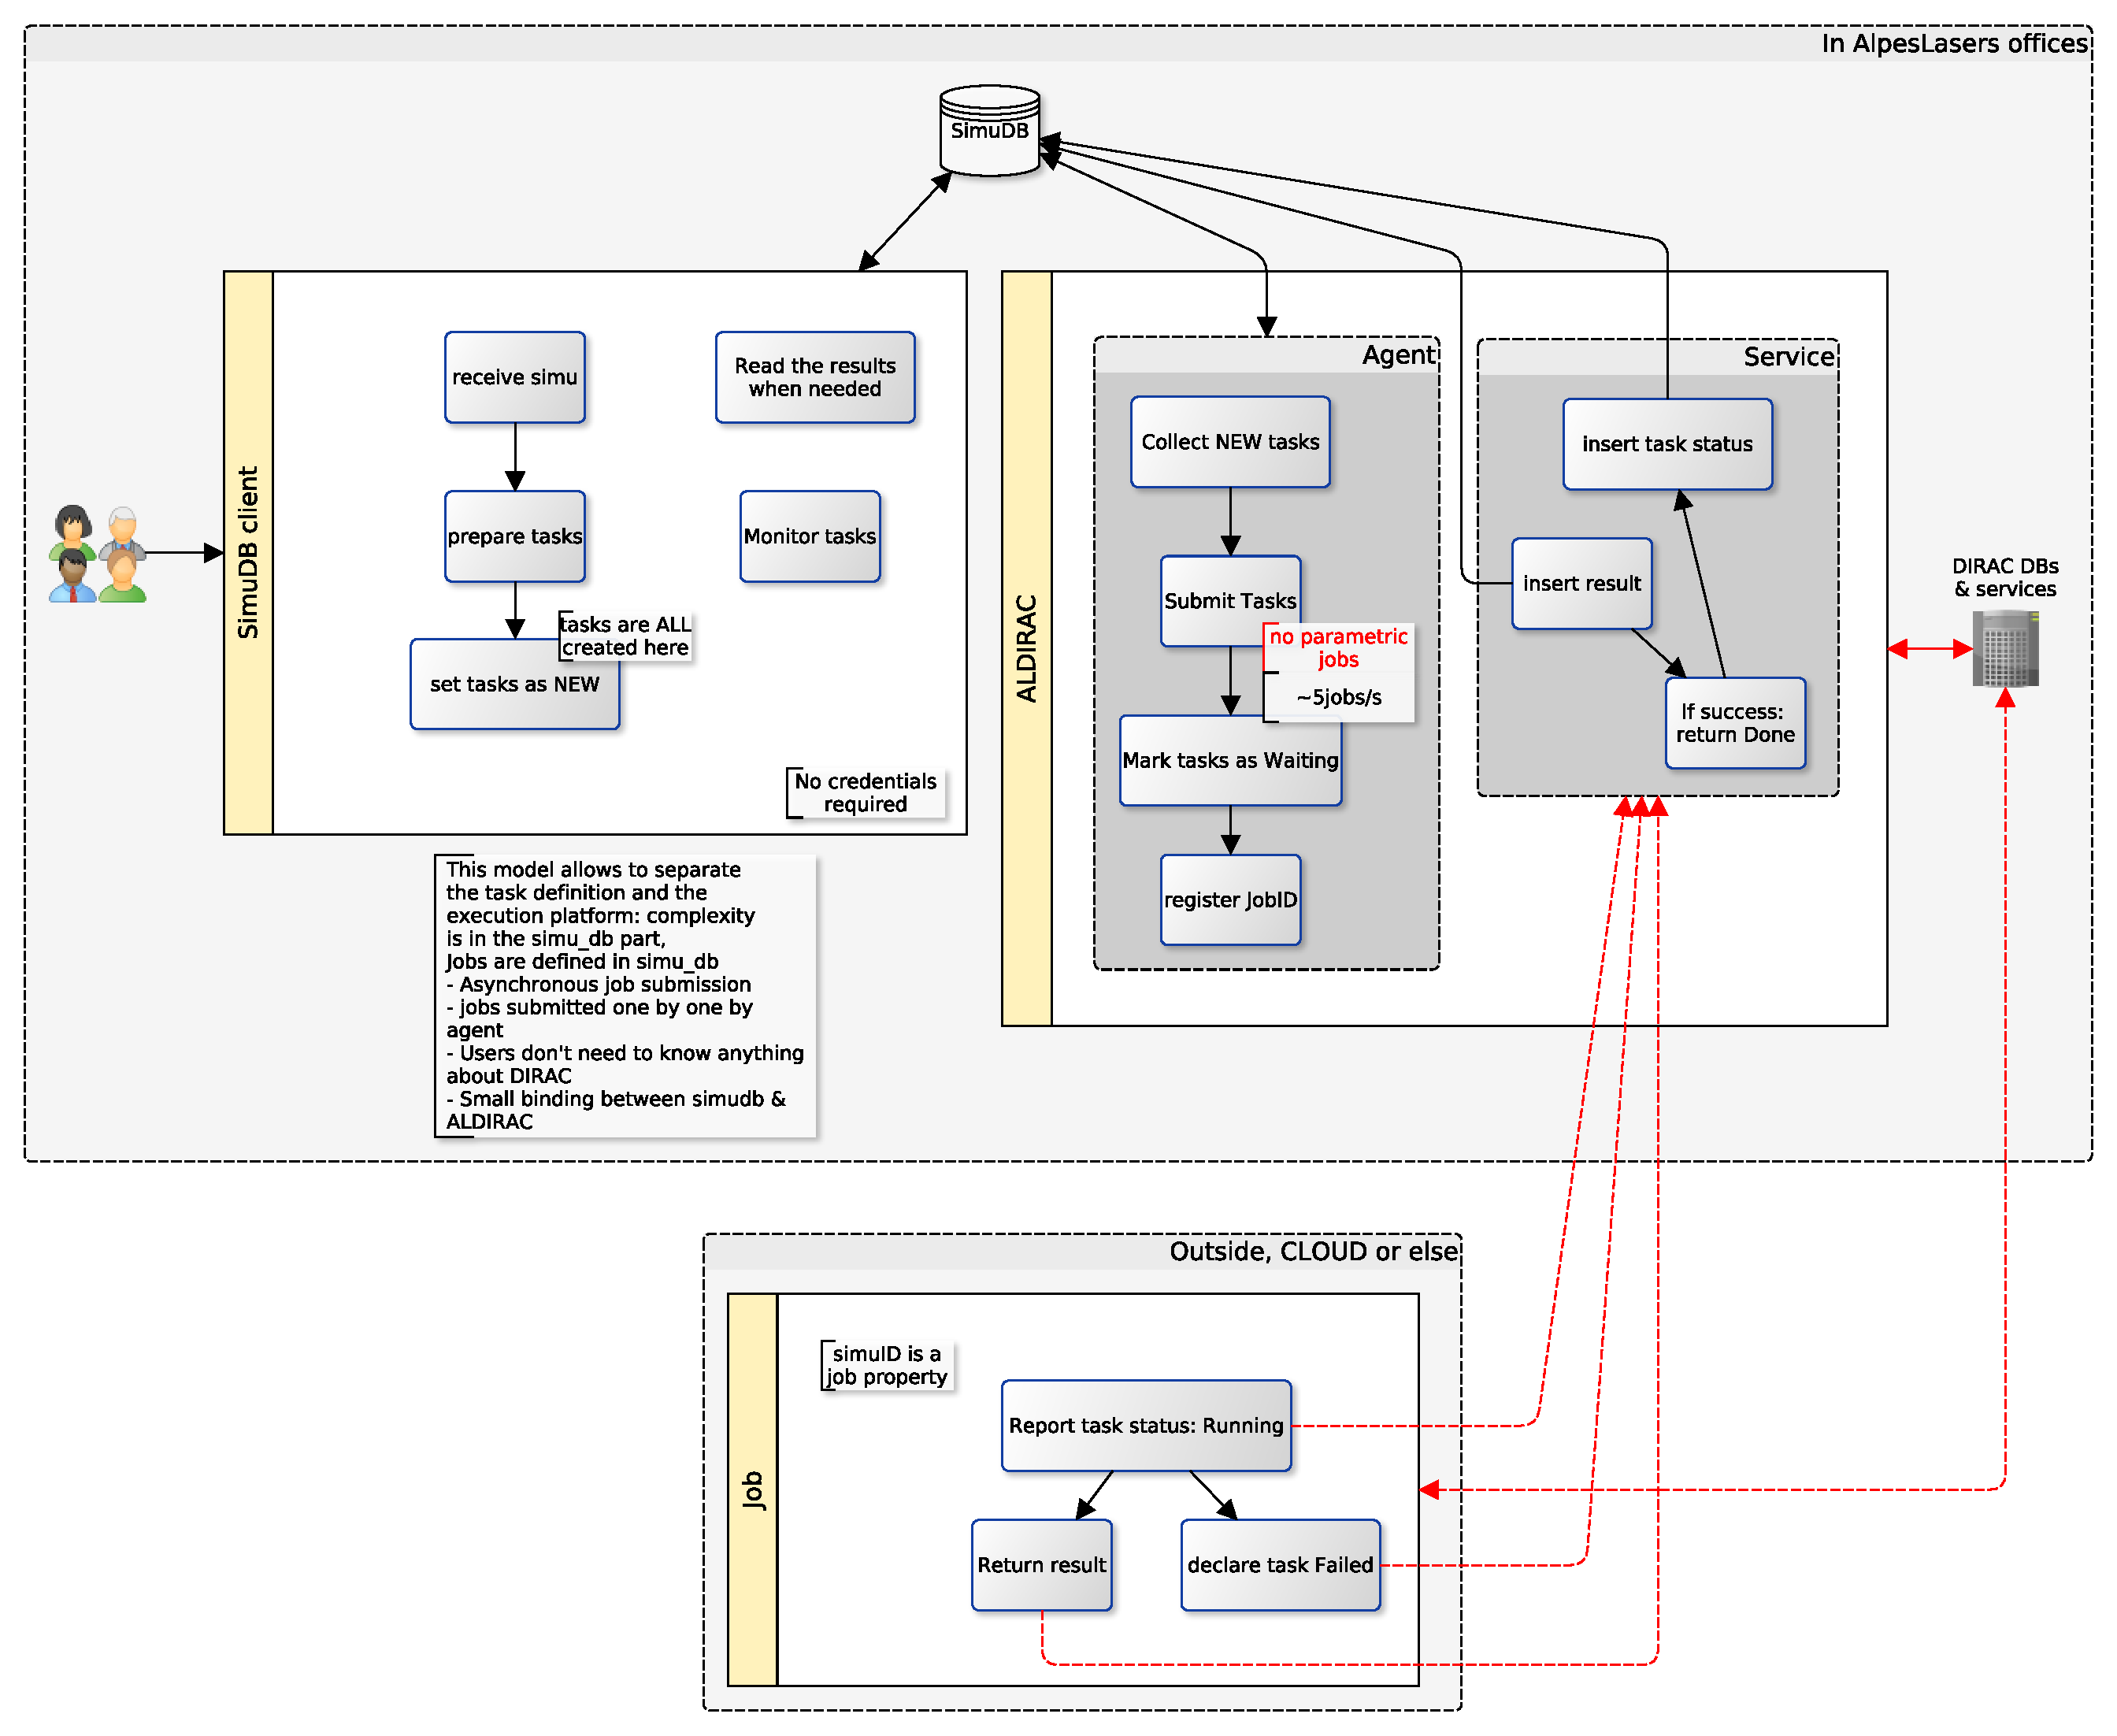
\includegraphics[width=\textwidth]{Architecture1.pdf}
\end{frame}

\section{Usage/cost report}
\begin{frame}
\frametitle{Usage}
\centering
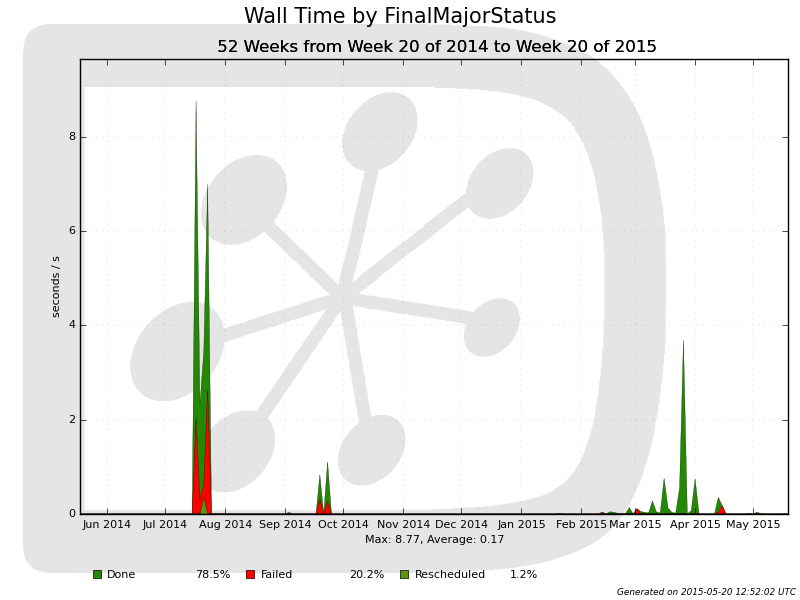
\includegraphics[width=\textwidth]{walltime.png}
\end{frame}

\begin{frame}
\frametitle{Costs}
\centering
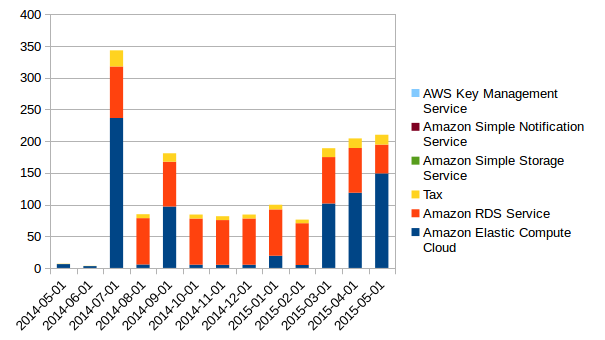
\includegraphics[width=\textwidth]{awscosts.png}
\end{frame}

\section{Comments}
\begin{frame}
\frametitle{Things that can hurt}
\begin{itemize}
\item Project leadership
\item project planning
\item project stability
\item Project usability
\end{itemize}
\end{frame}

\begin{frame}
\frametitle{Project leadership}
\begin{itemize}
\item Who is responsible?
\item Who is the contact person?
\item Who is responsible for what?
\end{itemize}
\end{frame}

\begin{frame}
\frametitle{Project planning}
\begin{itemize}
\item Where are written the development plans?
\item Where are the specs for the required changes?
\item Can we stick to plans?
\end{itemize}
\end{frame}

\begin{frame}
\frametitle{Project stability}
Ensure 1-year stability:
\begin{itemize}
\item Need utilities to migrate
\item Need ``guarantee'' that systems work
\item Public reports for run quality (CI reports)
\end{itemize}
\end{frame}

\begin{frame}
\frametitle{Project usability}
Required:
\begin{itemize}
\item Better deploy/install tools: can we use setup.py?
\item pyOpenSSL?
\item 'Standard' tools e.g. SimpleXMLRPCServer allows keyword args, function doc lookup (self documented client)
\item Exceptions
\item PEP8
\end{itemize}
Web platform: why not django?
\end{frame}

\section{Prospects}
\begin{frame}
\frametitle{Prospects}
Submitted DIRAC abstract to

\centering

\includegraphics[width=\textwidth]{europython-2015-logo-white-bg.png}
\end{frame}

\end{document}